

\chapter{Literature Review}  

\section{Introduction}
There has been many advancement....


\section{Large Language Models (LLM)}
Natural language processing (NLP) has always been an intricate field because of the complexity of how humans communicate. The meaning of a message
can vary because of homonyms, tone, context, and other factors that affect the message delivered; these are some challenges computers face when trying
to replicate or learn text communication and expressions.  However, this changed with the introduction of Large Language Models (LLM) \cite{naveed2024comprehensiveoverviewlargelanguage}.
These models are trained with large amounts of data to replicate human-like patterns or generate text based on statistical relationships between words, and all
was made possible because of transformers \cite{vaswani2023attentionneed}. Previous NLP techniques such as Recurrent Neural Network (RNN) and
Long-Short Term Memory (LSTM) could understand a sentence context in the short term. However, these struggle when trying to understand longer texts.
In contrast, transformers architecture, seen in Figure \ref{transformer}, differs from others because it uses self-attention.

\begin{figure}[!hb]
    \centering
        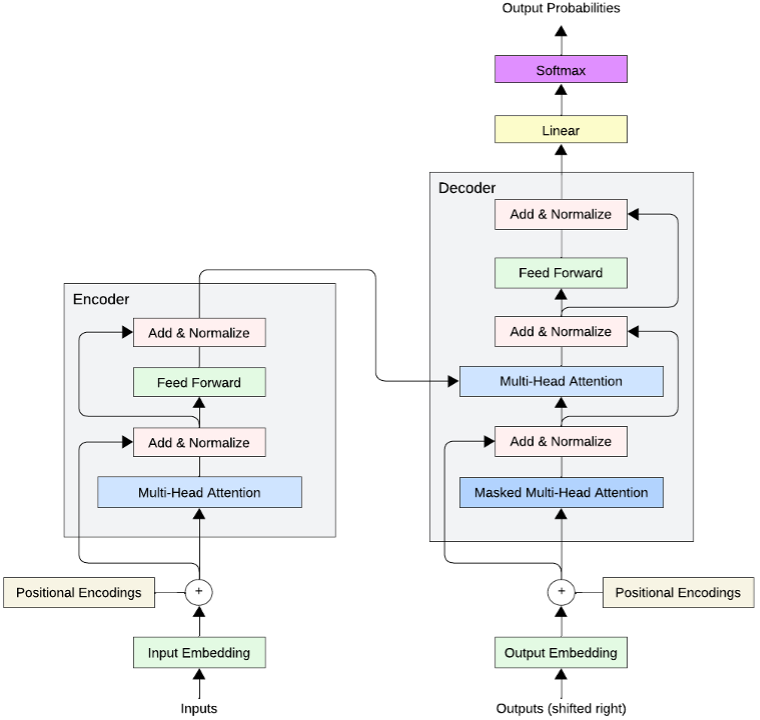
\includegraphics[width=1\linewidth]{images/transformers_architecture.png}
        \caption{The Transformer Architecture}
        \label{transformer}
\end{figure}

This self-attention finds dependencies between all words in a text, short and long-term. The process of this starts by turning words into tokens. A token can be a word,
subword, individual letter, or a sequence of words mapped to an embedding. The embedding is the vector representation of a token in high-dimension space; its size
depends on how much information it stores about the token. Now, self-attention finds relationships between all tokens and gives them an attention score, measuring
the relevance of a token to others. Transformers uses the scores to generate a final representation of each token. This process depends on how the models make a token.
The tokenization strategy is determined by the preprocessing stage, and influenced by the embedding and model architecture. The embedding impacts the strategy
because of its dimensionality, the amount of information encoded, and the model's sequence length limitations. In Figure \ref{transformer},  we can see an encoder and a
decoder in the transformers architecture. Based on that, there are different LLM architectures: decoder-only, encoder-only, and encoder-decoder. Each one has advantages
for specific tasks and limitations for others.

\begin{figure}[!hb]
    \centering
        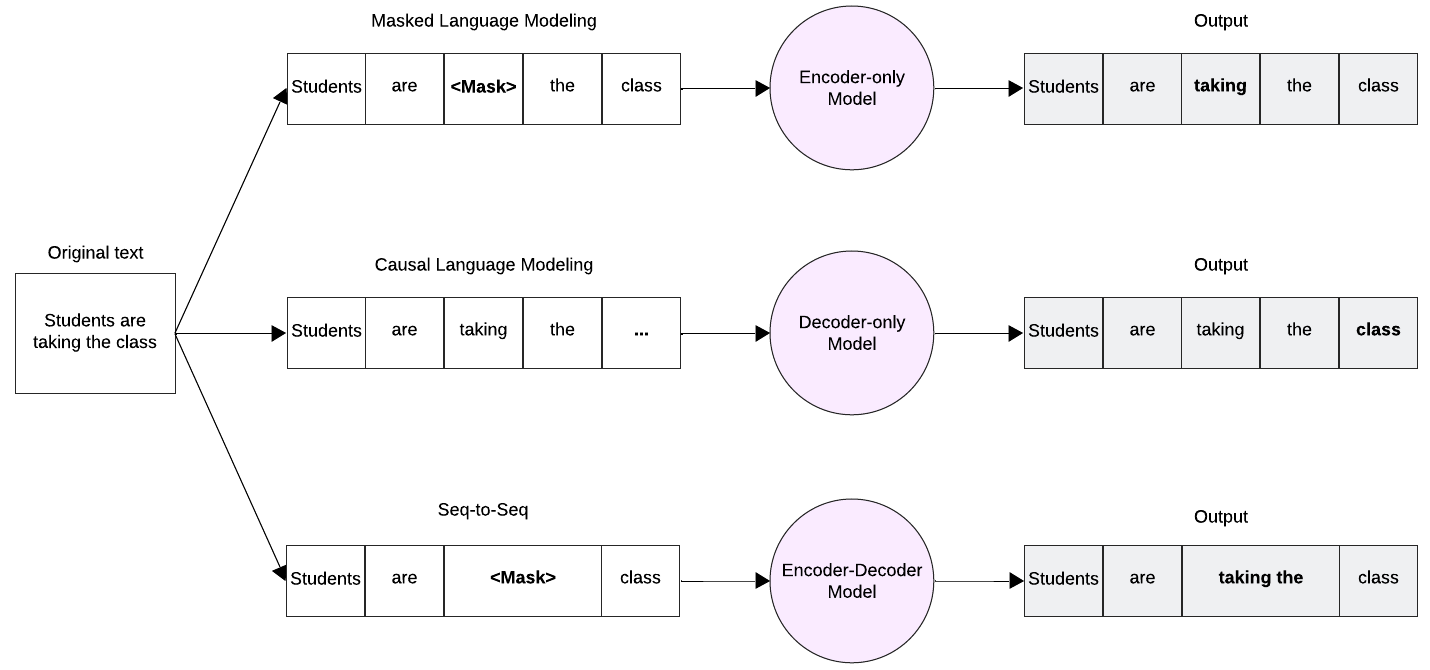
\includegraphics[width=1\linewidth]{images/LLM_Arch_text_generation.png}
        \caption{LLM Architecture and Comparison}
        \label{text_generation}
\end{figure}

\subsection{Decoder-only models}
Decoder-only models predict the next word based on the previous context, thus being unidirectional models. The model achieves this by taking a text or prompt as input and returning 
a first word. For each subsequent word, the model uses the previously generated text as input to predict the next word, continuing until it produces a coherent output. In Figure \ref{text_generation},
the model predicts the last word based the previous context. Because of their ability to predict sequences of texts, they are frequently employed in tasks like summarization and text generation. Models
that perform those task are also called causal language modeling (CLM), because they predict new tokens not found in the input. Compared to the other architectures, these models are massive
in size. Because of their sizes, these are not very practical or cost-effective for daily usage. These are the most commonly known models, such as GPT-3 \cite{DBLP:journals/corr/abs-2005-14165},
Mistral \cite{jiang2023mistral7b}, and LLaMa \cite{touvron2023llamaopenefficientfoundation}.

\subsection{Encoder-only models}
This type of model predicts by masking specific words in a sentence. Said masking helps them understand the meaning or relation of the masked word based on context. They are bi-directional,
which means they take the context before and after the masking to evaluate the word. The example in Figure \ref{text_generation} shows a sentence with a word mask and being inputted to
the encoder LLM; the model predicts the missing word by using the surrounding text. That is why they tend to perform well at classification and sentiment analysis but are not optimal for text
generation. Said model are called masked language models (MLM). In contrast to other architectures, these models are relatively small. Some examples of encoder-only LLM are BERT
\cite{DBLP:journals/corr/abs-1810-04805} and RoBERTa \cite{liu2019robertarobustlyoptimizedbert}.

\subsection{Encoder-Decoder models}
Encoder-decoder models combines masking and text generation. The way the work is by masking sequence of texts and using the context around it to make a prediction. As seen
in Figure \ref{text_generation}, they can mask more than one word from the original inputted text. Because the model generates sequences of texts, it is commonly used for translation
and question and answer. It is know that translating from one language to another is not possible using a word by word translation; one must understand the entire sequence to not loss context.
To have an optimal model, both encoder and decoder must be trained for the task one wishes to achieve. Depending on the task, it can be harder to train compared to the other types of architectures.
Bart \cite{lewis2019bartdenoisingsequencetosequencepretraining} and T5 \cite{chung2022scalinginstructionfinetunedlanguagemodels} are example of encoder-decoder LLMs.


\subsection{Classification tasks}
Large Language Models use different learning methods to train. Such methods include zero-shot, one-shot, and few-shot learning. As the name implies, zero-shot learning is training a model without
previous knowledge of the data; it is learning from scratch. One-shot learning is a method that receives one example as input and tries to generalize from that example. The final method uses
multiple examples to find a pattern between them. 

In Figure \textbf{[IMAGE]}, we can see an example of zero-shot learning. This LLM has no previous knowledge of the task that it must perform. Nonetheless, the model used, GPT-3, has the 
advantage that it can follow instructions when redacted clearly. Here, we tell the model that it must act as a medical expert and identify if a message is health-related and why it is classified that way. 
Also, the result must follow a specific format. This process of instructions is called prompt engineering. Prompting does not retrain or adjust the model parameters. Thus, it does not always have optimal results.  

 \textbf{[FIGURE]}


Moreover, LLMs that completed training with no additional modifications are known as based models. The response from this model will most likely make no sense with the premises it receives.
This happens because the model is trained on excessive texts to find patterns between them, but this pattern might not be on par with the input. For the model to return a coherent response, it must go
through a finetuning process. Finetuning consists of making a model perform specific tasks, such as chatting, summarization, chatbots, and others. To finetune a model, it must undergo another training process, but now the training data relates to the tasks it will perform. 

The authors in \textbf{[REFERENCE]} created a model to understand images and give a text description or a combination of text and image. The model was trained on images and captions of those
images using zero-shot. Their resulting model was used to create a chatbot that identifies images, answers questions, or gives visual examples about them. Another experiment was \textbf{[REFERENCE]},
where the authors trained a model to identify sentiments on financial market decisions. The advantage of in-context learning of the model resulted in a 70\% accuracy on sentiment prediction,
failing mostly on neutral posts. That experiment showed the problems that users face when they use social media to make decisions. They clarified the importance of not taking the model for granted
and how social media can cause a user to make a poor decision.  


\section{Misinformation in Social Media}
There are many sources in the world to find information about any topic. Nonetheless, many people use social media as their primary source and mostly take this information as truth without
validation. On occasion, these can be fake, misleading, or wrong. When this happens unintentionally or by lack of understanding of the topic, it is called misinformation. On the other hand,
when it is intentional to provide wrong information, this is known as disinformation. For simplification, both terms will be used interchangeably.

Misinformation has been dangerous during critical events like natural disasters or health crises. For instance, during the COVID-19 pandemic, falsehood arose saying that the vaccine had
microchips, which led many people to die [1] because they refused to get vaccinated out of fear. A problem with disinformation is that the audience does not always detect it. When misinformation
spreads and is not clarified early on, it can be confused as fact. Older audiences and people with less education are more likely to share and believe fake or misleading news \textbf{[REFERENCE]}. 

There has been various research on reducing the propagation of misinformation. Misinformation was seen as a game-theoretic in \textbf{[REFERENCE]}, where some players spread fake news, and others tried
to stop it. They created an agent at the network level to combat misinformation in a simulation. However, they could not conclude the efficiency of their model because of the lack of a pattern. On
the other hand, in \textbf{[REFERENCE]} the authors used LSTM and BERT to classify misinformation from the different news sources. They proved that BERT outperformed LSTM, achieving an accuracy of 64.88\% against 60.59\%. 
Another approach to detecting fake information was on \textbf{[REFERENCE]}, where they detected fake LinkedIn profiles. On this occasion, the dataset used for training included real and AI-generated profiles. They tested multiple
LLMs, but BERT resulted in the highest accuracy of 95.67\%. These investigations prove the efficiency of Large Language Models for Natural Language Processing in the misinformation field. Regardless,
none of these studies addresses health-related misinformation on social media.




% Misinformation link: \cite{9906925}

